% CS701 course project report — CVPR template (<= 6 pages, references excluded as usual).
% Compile on Overleaf with the CVPR 2026 author kit (cvpr.sty) or any recent cvpr/latex kit.
% Replace \teamID and author list; delete \draft notes before submission.
\documentclass[10pt,twocolumn,letterpaper]{article}

\usepackage[review]{cvpr}      % switch to {cvpr} (final) before submitting
\usepackage{graphicx}
\usepackage{amsmath,amssymb}
\usepackage{booktabs}
\usepackage{multirow}
\usepackage{enumitem}
\usepackage{xcolor}
\definecolor{cvprblue}{rgb}{0.21,0.49,0.74}
\usepackage[pagebackref,breaklinks,colorlinks,allcolors=cvprblue]{hyperref}

\def\paperID{teamNN} % <-- team number
\def\confName{CVPR}
\def\confYear{2026}

\newcommand{\dm}{\ensuremath{\Delta m}}
\newcommand{\todo}[1]{\textcolor{red}{[#1]}}

\title{Multi-Task Learning on SAR Images:\\A Frozen DINOv3 Backbone with LoRA and a Tiny-Object Detector}

\author{Member A\quad Member B\quad Member C\quad Member D\\
CS701, School of Computing and Information Systems, Singapore Management University\\
{\tt\small cs701-teamNN}
}

\begin{document}
\maketitle

%%%%%%%%% ABSTRACT
\begin{abstract}
We study multi-task learning on synthetic aperture radar (SAR) images: one model
must classify an image into nine scene classes and detect all of its objects,
half of which are smaller than a 16\,px ViT patch. Our final model keeps a
DINOv3 ViT-B/16 backbone frozen and adapts it with LoRA on every linear layer
plus the LayerNorms (23.8\,M trainable parameters). A shared feature pyramid
feeds a class head and a detector redesigned for tiny objects: NWD-based anchor
matching, small anchors at cell centres, and a three-stage Cascade R-CNN with
light class-agnostic heads. A post-processing stage scores boxes by the
detector probability combined with RPN objectness, applies per-class soft-NMS,
averages the cascade stages' boxes, and lets the detections inform the image
class. On the Codabench validation leaderboard the model reaches
macro-F1 95.06 / mAP 45.62, i.e.\ $\dm = +38.23$ against the ViT + LoRA
reference, above the over-budget full fine-tuning reference ($+13.5$). We also
report a lighter single-shot family (YOLO + DINOv3 feature fusion, 31\,M
parameters) that reaches about $+21$: a useful efficiency comparison.
Ablations on held-out data quantify what each component adds.
\end{abstract}

%%%%%%%%% 1 INTRODUCTION
\section{Introduction}
\label{sec:intro}

Synthetic aperture radar (SAR) images look like photographs but are not:
each pixel is the strength of a microwave echo, so images are 8-bit gray,
grainy with speckle, and have statistics unlike RGB photographs. The CS701
assignment asks for \emph{one} model that reads one SAR image and produces
two outputs: the image's class (one of nine) and a bounding box, class and
score for every object in it --- all boxes share the image's class. The
leaderboard ranks models by \dm, the mean relative gain of macro-F1 and COCO
mAP over a reference model (ViT-B/16 + LoRA). The budget is tight: at most
130\,M parameters in total and 40\,M trainable, one model, no ensembles or
test-time augmentation, and each image seen once at $\le 512\times512$ pixels.

Two properties of the data shape the design. First, \emph{objects are tiny}:
the median box side is 15\,px and 52.6\,\% of all boxes are smaller than one
$16{\times}16$ ViT patch, so a stride-16 backbone loses them. Second,
\emph{pretraining matters more than architecture}: the reference from-scratch
runs score $\dm \approx -20$ while LoRA scores 0.

Our approach is simple in outline: spend the trainable budget where it pays.
We freeze a DINOv3 ViT-B/16 --- a strong generic self-supervised backbone ---
and train LoRA rank-32 adapters on all linear layers plus the LayerNorms
(23.8\,M trainable). On top of the shared backbone we put (i) a light
classification head on the mean token and (ii) a detector rebuilt for tiny
objects: a ViTDet simple feature pyramid, an RPN that matches anchors by
normalized Wasserstein distance (NWD) rather than IoU alone with small anchors
centred on the pixel grid, and a three-stage Cascade R-CNN with light
class-agnostic heads. Boxes are then rescored by detector probability times
RPN objectness, suppressed by per-class soft-NMS, and corrected for a measured
sub-pixel annotation bias; the image class fuses the classifier's and the
detector's confidences.

\textbf{Results.} On the Codabench validation leaderboard the model reaches
macro-F1 95.06 and mAP 45.62 ($\dm = +38.23$), against the reference's 93.31 /
26.13 and the over-budget full fine-tuning upper bound ($+13.5$ test). Each
component is ablated on stratified holdouts of the training split; the largest
gains come from the DINOv3 backbone ($+8$), wider LoRA ($+10$), and the
tiny-object detector changes ($+13$). For efficiency we also train a second
family --- YOLO detectors with DINOv3 feature fusion --- reaching
$\dm \approx +21$ at 31\,M parameters.

%%%%%%%%% 2 RELATED WORK (short)
\section{Related work}
\label{sec:related}
\textbf{Efficient adaptation.} LoRA~\cite{hu2022lora} trains a low-rank update
of frozen weights; mixtures of LoRA experts with task routing
(MTLoRA~\cite{agiza2024mtlora}, MLoRE) are the reference's own extension. We
keep single LoRA but widen it to all linear layers and train the norms.
\textbf{Small-object detection.} Tiny boxes break IoU-based assignment
(NWD~\cite{wang2021nwd}) and need fine features (ViTDet~\cite{li2022vitdet},
ViT-Adapter~\cite{chen2023vitadapter}) and cascade refinement~\cite{cai2018cascade}.
\textbf{Multi-task learning.} We share one frozen backbone between a class head
and a detector, and let each task's outputs correct the other at inference
(detection-informed classification).

%%%%%%%%% 3 METHOD
\section{Method}
\label{sec:method}

Figure~\ref{fig:model} shows the model. One forward pass at $512\times512$
produces the class and the boxes.

\begin{figure}[t]
\centering
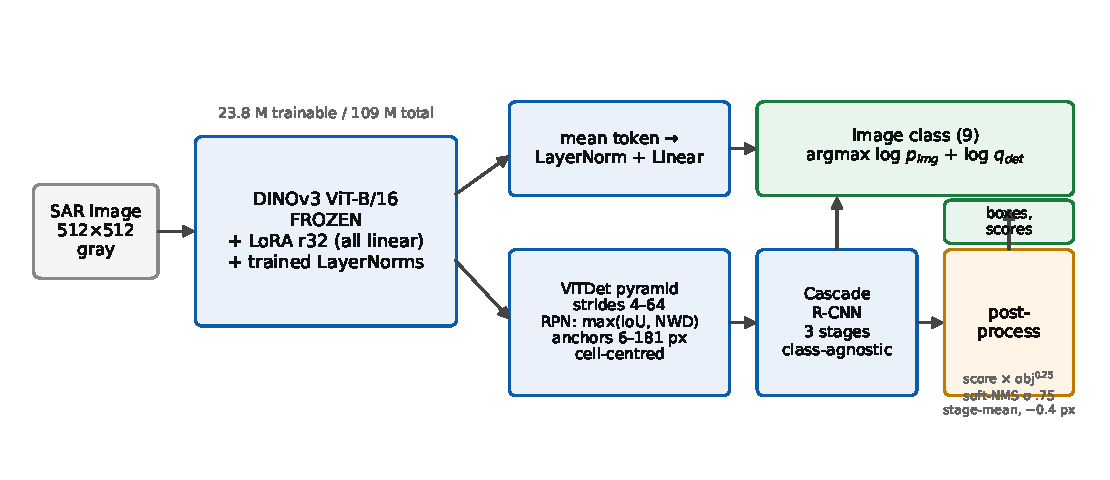
\includegraphics[width=\linewidth]{figures/model_diagram.pdf}
\caption{The model: frozen DINOv3 ViT-B/16 + LoRA (rank 32, all linear layers,
trained LayerNorms). Mean token $\rightarrow$ LayerNorm+Linear $\rightarrow$
image class. ViTDet feature pyramid $\rightarrow$ RPN (NWD matching, small
cell-centred anchors) $\rightarrow$ 3-stage class-agnostic Cascade R-CNN.
Post-processing fuses the two outputs.}
\label{fig:model}
\end{figure}

\subsection{Backbone: frozen DINOv3 + LoRA}
\label{sec:backbone}
The backbone is timm \texttt{vit\_base\_patch16\_dinov3.lvd1689m}, a ViT-B/16
self-distilled on 1.7\,B web images (no SAR). The patch embedding sums its RGB
weights into one gray channel; inputs are normalised with the train-set mean
and std (0.2526 / 0.2133) rather than ImageNet's. The backbone is frozen.
Trained: LoRA rank 32 ($\alpha = 64$) on \texttt{attn.qkv}, \texttt{attn.proj},
\texttt{mlp.fc1}, \texttt{mlp.fc2} of all 12 blocks, plus every LayerNorm ---
23.8\,M trainable parameters (109\,M total; limits 130\,M / 40\,M). LoRA trains
at $3\times$ the head learning rate ($3\mathrm{e}{-4}$ vs $1\mathrm{e}{-4}$).

\subsection{Two heads on one backbone}
\textbf{Classification} reads the mean of the $32\times32$ patch tokens
through LayerNorm + Linear --- deliberately simple; attention pooling and CLS
concatenation were not better on our holdout.
\textbf{Detection} builds a ViTDet simple feature pyramid from the stride-16
token map (strides 4, 8, 16, 32, 64, 256 channels), then a Faster R-CNN-family
detector modified for tiny objects:

\begin{itemize}[leftmargin=1.1em,itemsep=1pt,topsep=2pt]
\item \textbf{NWD matching.} For an 8\,px box, a 2\,px offset makes IoU
$\approx 0$, so IoU-based anchor matching starves tiny objects of positives.
The RPN matches anchors by $\max(\mathrm{IoU}, \mathrm{NWD})$ with the
normalized Gaussian Wasserstein distance ($C{=}8$).
\item \textbf{Small anchors at cell centres.} Sizes 6--181\,px over the five
levels, centred at $(i{+}0.5)\times$ stride --- the centre of the image region
each pyramid cell covers.
\item \textbf{Cascade R-CNN.} Three stages (IoU 0.5/0.6/0.7) with light
class-agnostic heads (4.3\,M each; all boxes of an image share one class, so
per-class regression buys little) and aligned RoIAlign.
\end{itemize}

\subsection{Post-processing (single forward pass)}
\label{sec:post}
All post-processing uses only the model's own outputs for the same forward
pass --- one model, no TTA. Box score $=$ detector probability $\times$
RPN objectness$^{0.25}$; per-class Gaussian soft-NMS ($\sigma{=}0.75$); boxes
are the mean of the three cascade stages' outputs; a constant $-0.4$\,px shift
removes a systematic annotation bias measured on the holdouts; every image
keeps at least 30, at most 100 boxes at threshold $10^{-5}$. The image class
is $\arg\max_c [\log p_{\mathrm{img}}(c) + \log q(c)]$, $q(c)$ the highest
detector probability of class $c$.

\subsection{Training protocol}
\label{sec:train}
Batch 16, AdamW ($\mathrm{wd}\,{=}\,0.05$), one warmup epoch, cosine to 0,
bf16, flips only (SAR overhead has no canonical ``up''; rotations and
copy-paste did not help --- Section~\ref{sec:negative}). The reported model
trains 100 epochs on all 9\,392 labelled images; model selection used a
stratified 80/10/10 split of train. Two RTX 6000 Ada, 3.5\,h, peak 38\,GB.

%%%%%%%%% 4 EXPERIMENTS
\section{Experiments}
\subsection{Setup}
\textbf{Data.} 9\,392 labelled SAR train images with 32\,533 boxes
(74.5\,\% at $512^2$, 24.7\,\% at $256^2$, the rest odd sizes; per-class image
counts 443--1\,355 but box counts 919--8\,625), 1\,426 unlabelled val and
2\,065 test images (Codabench).
For model selection we hold out a stratified 10\,\%+10\,\% of train as local
val/test (7\,512/940/940 images, seed 0); a 5-fold split cross-checks
choices. Our local holdout systematically \emph{over}-estimates Codabench
(V2: local mAP 48.9 vs 45.6 leaderboard), so local numbers are used only to
rank designs.

\textbf{Metric.} $\dm = 100 \times \frac12\big[\frac{\mathrm{F1} -
\mathrm{F1}_{ref}}{\mathrm{F1}_{ref}} + \frac{\mathrm{mAP} -
\mathrm{mAP}_{ref}}{\mathrm{mAP}_{ref}}\big]$ with
$\mathrm{F1}_{ref}{=}93.31$, $\mathrm{mAP}_{ref}{=}26.13$ (val). One run of a
configuration varies by about $\pm 1$ \dm; differences under $\sim$1.5 are
noise.

\subsection{Main result}
\begin{table}[t]
\centering\footnotesize
\setlength{\tabcolsep}{4pt}
\begin{tabular}{@{}lccc@{}}
\toprule
Model & macro-F1 & mAP & \dm \\
\midrule
Reference (ViT+LoRA, our run) & 93.3 & 26.1 & 0 \\
Full FT (over budget) & 94.4 & 32.0 & +11.8 \\
YOLO11-s improved (48 ep) & 93.08$^\dagger$ & 36.93$^\dagger$ & +20.53$^\dagger$ \\
DINO-YOLO26-s (100 ep) & 93.7 & 37.2 & $\approx$+21 \\
\textbf{Ours (V2, 100 ep)} & \textbf{95.06}$^\dagger$ & \textbf{45.62}$^\dagger$ & \textbf{+38.23}$^\dagger$ \\
\bottomrule
\end{tabular}
\caption{Codabench validation leaderboard ($^\dagger$) or local val. The
reference full fine-tuning exceeds the 40\,M trainable budget; shown as an
upper bound.}
\label{tab:main}
\end{table}

Table~\ref{tab:main} puts the model next to the references and the team's
single-shot line. The 45.6 val mAP is 19.5 points over the LoRA reference and
13.6 over the over-budget full fine-tuning reference --- most of \dm{} comes
from detection.

\subsection{What each part adds}
\begin{table}[t]
\centering\footnotesize
\setlength{\tabcolsep}{4pt}
\begin{tabular}{@{}llcc@{}}
\toprule
Run & change (cumulative) & ep & local \dm \\
\midrule
E00 & reference ViT-B/16 IN-21k + LoRA r16 & 24 & 0 \\
E01 & + DINOv3-B backbone & 24 & +8.1 \\
E04r & + LoRA r32 all-linear + norms & 24 & +18.1 \\
D1/D2 & + Cascade / + NWD, small anchors & 24 & +21.0 / +19.7 \\
C36 & + both & 36 & +31.3 \\
C48 & + both, longer & 48 & +38.6 \\
V2 & same, 100 ep, train+val & 100 & +38.2 (LB) \\
\bottomrule
\end{tabular}
\caption{Ablation ladder on the local holdouts (seed noise $\approx\pm1$ \dm;
LB $=$ Codabench leaderboard).}
\label{tab:ablation}
\end{table}

Table~\ref{tab:ablation} (Figure~\ref{fig:ladder}) is the cumulative ladder.
DINOv3 over ImageNet ViT is
the single biggest backbone gain; widening LoRA to all linear layers and
training norms nearly doubles it again. On the detector side, NWD matching +
small anchors and the cascade are complementary ($+13$ combined at 36 epochs),
and long training keeps paying until about epoch 100.

\begin{figure}[t]
\centering
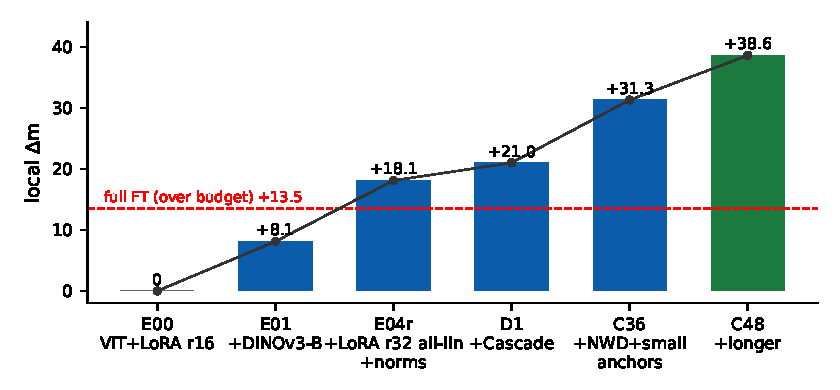
\includegraphics[width=\linewidth]{figures/ablation_ladder.pdf}
\caption{Local \dm{} of the cumulative ablation ladder (stratified holdout of
the train split). The dashed line is the over-budget full fine-tuning
reference.}
\label{fig:ladder}
\end{figure}

\textbf{Post-processing} (\S\ref{sec:post}) adds $\approx+2$--3 mAP in total
on the same frozen outputs: soft-NMS with objectness rescoring
($+1.3$--1.8), stage-mean boxes ($+0.3$--0.5), the $-0.4$\,px correction
($+0.4$--0.7), and the 30-box floor ($+0.1$).

\subsection{Per-class and size analysis}
\begin{figure}[t]
\centering
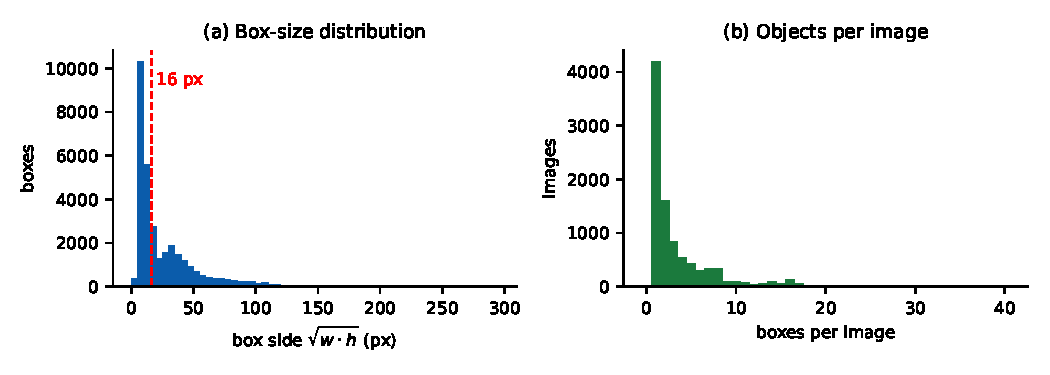
\includegraphics[width=\linewidth]{figures/box_stats.pdf}
\caption{Detection targets are tiny: (a) 52.6\,\% of all boxes are under
16\,px --- below one ViT patch --- and 19.5\,\% under 8\,px; (b) images hold
1--41 objects (45\,\% a single box).}
\label{fig:boxes}
\end{figure}
\todo{Table: per-class AP and AP by box size (tools/size\_ap.py). Weak
classes: bridge, playground, wind\_turbine; per-class AP from V2 run.}

\subsection{A lighter single-shot alternative}
\label{sec:yolo}
For efficiency we also train YOLO12/26-s detectors whose backbone receives
DINOv3 ViT-S features through zero-initialised $1\times1$ convolutions
(31\,M parameters, all trainable). The image class is read from the
detections (highest total score per class). After 100 epochs DINO-YOLO26-s
reaches local test \dm{} $+21.3$ (F1 93.9, mAP 37.1) --- 17 points behind the
two-stage model on mAP but at a third of the parameters and a single-shot
latency. The DINO fusion adds $+3$--4 mAP over the plain YOLO26-s.

%%%%%%%%% 5 ANALYSIS
\section{Analysis}
\subsection{What did not work}
\label{sec:negative}
Overlapping stride-8 patches ($\sim$2.6$\times$ tokens) helped bridge,
playground and wind turbine but cost oil tank ($-0.4$ mAP overall); LoRA rank
64, D4 rotations, copy-paste augmentation, a multi-level ViT neck, ConvNeXt
backbones and Mona adapters did not beat the recipe either and were dropped.
A classification head on the DINO-YOLO features raised F1 by +3--4 but cost
$\sim$1.5 mAP, so the detector-vote classification was kept.

\subsection{Efficiency}
\begin{table}[t]
\centering\small
\begin{tabular}{@{}lccc@{}}
\toprule
 & total & trainable & inference \\
\midrule
Reference LoRA & 107 M & 21.0 M & --- \\
DINO-YOLO26-s & 31.9 M & 31.9 M & --- \\
\textbf{Ours} & \textbf{109.0 M} & \textbf{23.8 M} & \textbf{15 ms/img} \\
\bottomrule
\end{tabular}
\caption{Parameter budget and cost. Trainable parameters include the heads.
Inference: bf16 on one RTX 6000 Ada.}
\label{tab:eff}
\end{table}

\subsection{Submission protocol}
Phase-1 submissions were scored on the local holdouts first, then uploaded
(daily limit 5). For Phase 2 we retrain the selected recipe on all labelled
data at the epoch count chosen on the holdout (100), and reserve one of the
two allowed submissions for a checkpoint-averaged variant \todo{or: the
second model the team chooses}.

%%%%%%%%% 6 CONCLUSION
\section{Conclusion}
On SAR imagery, a generic self-supervised backbone left frozen and adapted by
wide LoRA beats the ImageNet reference by a wide margin; the remaining, larger
gain comes from rebuilding the detector for sub-patch objects (NWD matching,
small cell-centred anchors, cascade refinement, fused post-processing). Within
the 40\,M-trainable budget the model more than doubles the reference's
leaderboard score.

{\small
\bibliographystyle{ieeenat_fullname}
\bibliography{main}
}

\end{document}
